%\documentclass[wsdraft]{ws-procs11x85}
%\documentclass[square]{ws-procs11x85}
\documentclass{ws-procs11x85}
\usepackage{hyperref}
\begin{document}

\title{TRANSFER LEARNING FOR HUMAN PHENOTYPE ONTOLOGY TERMS}

\author{BEN KOMPA}

\address{UNC Chapel Hill,\\
E-mail: kompa@live.unc.edu\\}



\bodymatter

\section{The Problem: A Reminder}
All the code for this project is available here: \\ \href{https://github.com/bkompa/hpo}{https://github.com/bkompa/hpo}\\ \\ 
The goal of this project is to automatically tag electronic medical records with HPO terms. Because of a lack of labeled EMRs, we are using PubMed abstracts that are labeled with HPO terms. After training a learning method on the PubMed abstracts, we will apply them to EMRs and see if the learning can be transferred. 
An outline of the project:
\begin{itemize}
\item Select the PubMed articles with HPO terms (Completed)
\item Determine a viable learning method to tag PubMed articles (In Progress)
\item Apply the trained learning method to EMRs 
\end{itemize}

\section{Selecting PubMed Articles}

I downloaded the PubMed Open Access subset of PubMed abstracts, which was about 800,000 articles. While Inbar scraped PubMed for abstracts labeled with HPO terms. I then joined the two tables together to make our data set of 157,473 articles tagged with 1,307 different HPO terms. The next step was to look at the number of terms per article and the number of articles per term. If a term did not have sufficient coverage in the data set, it would be nearly impossible to tag future articles with that term. 



\begin{center}
  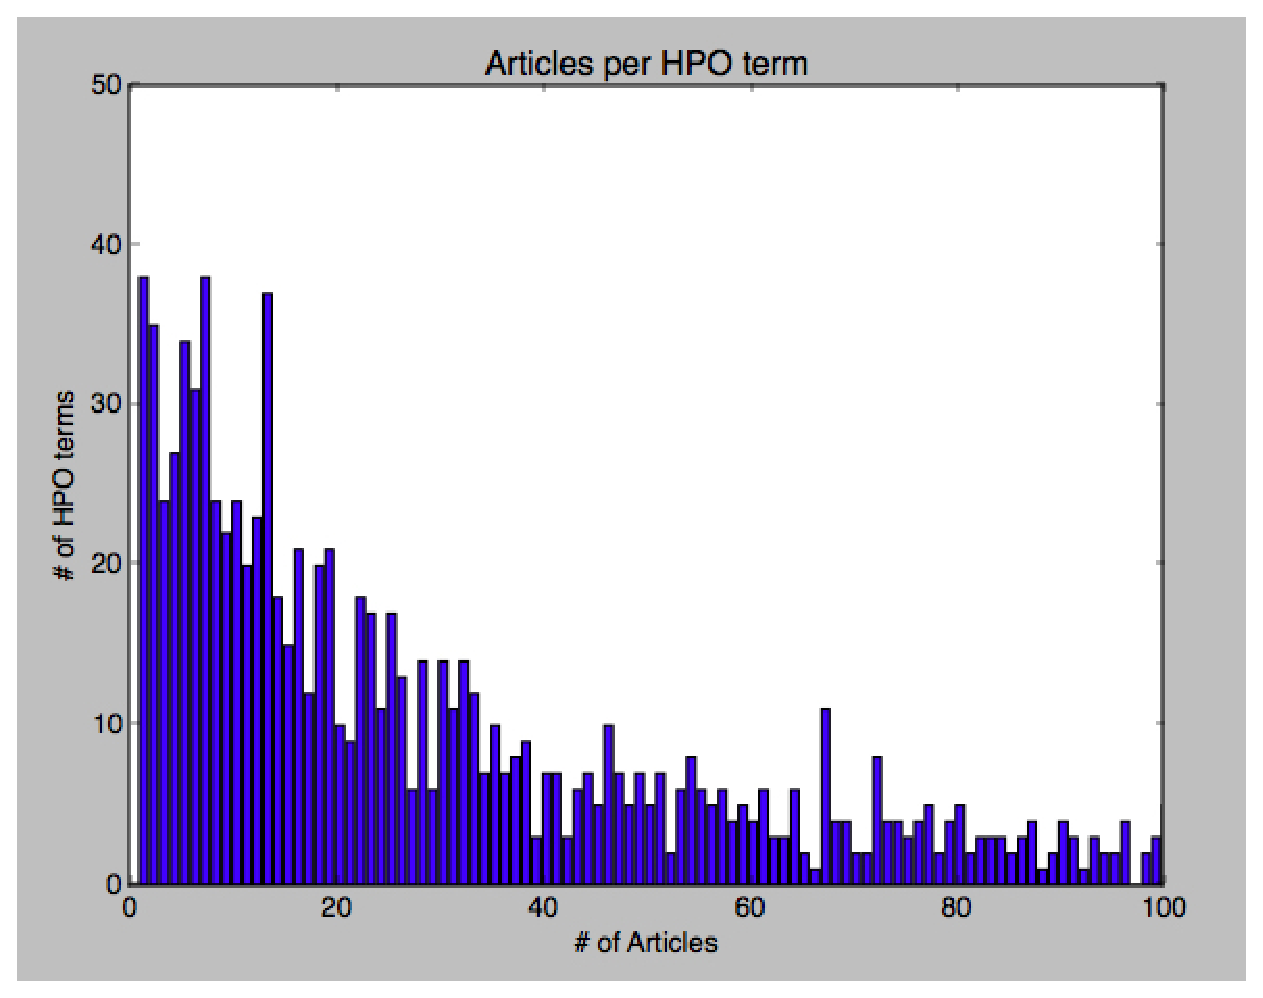
\includegraphics[width=8cm]{hpo-article}\\
 \small \textit{Fig 1.} This is a zoom in on the distribution of articles per HPO term. To determine the number of HPO terms that have at least \textit{X} articles, sum the Y-axis values from \textit{X} and above. 
\end{center}

\begin{center}
  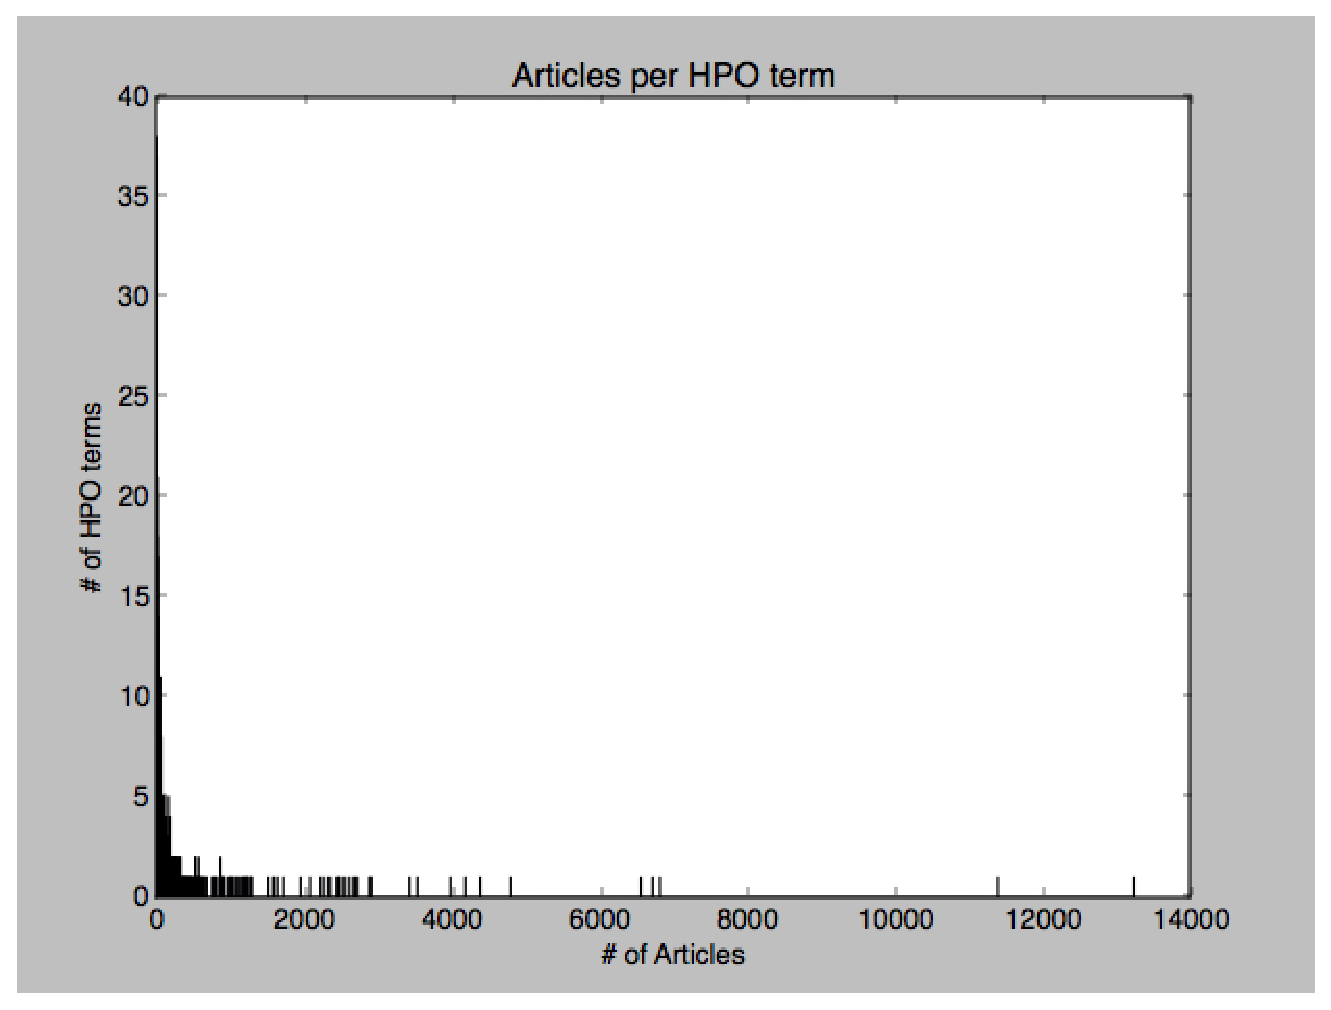
\includegraphics[width=8cm]{hpo-article-zoomout}\\
 \small \textit{Fig 2.} This is the whole distribution of articles per HPO term. The HPO term with the most articles is the term for breast cancer. 
\end{center}

\begin{center}
  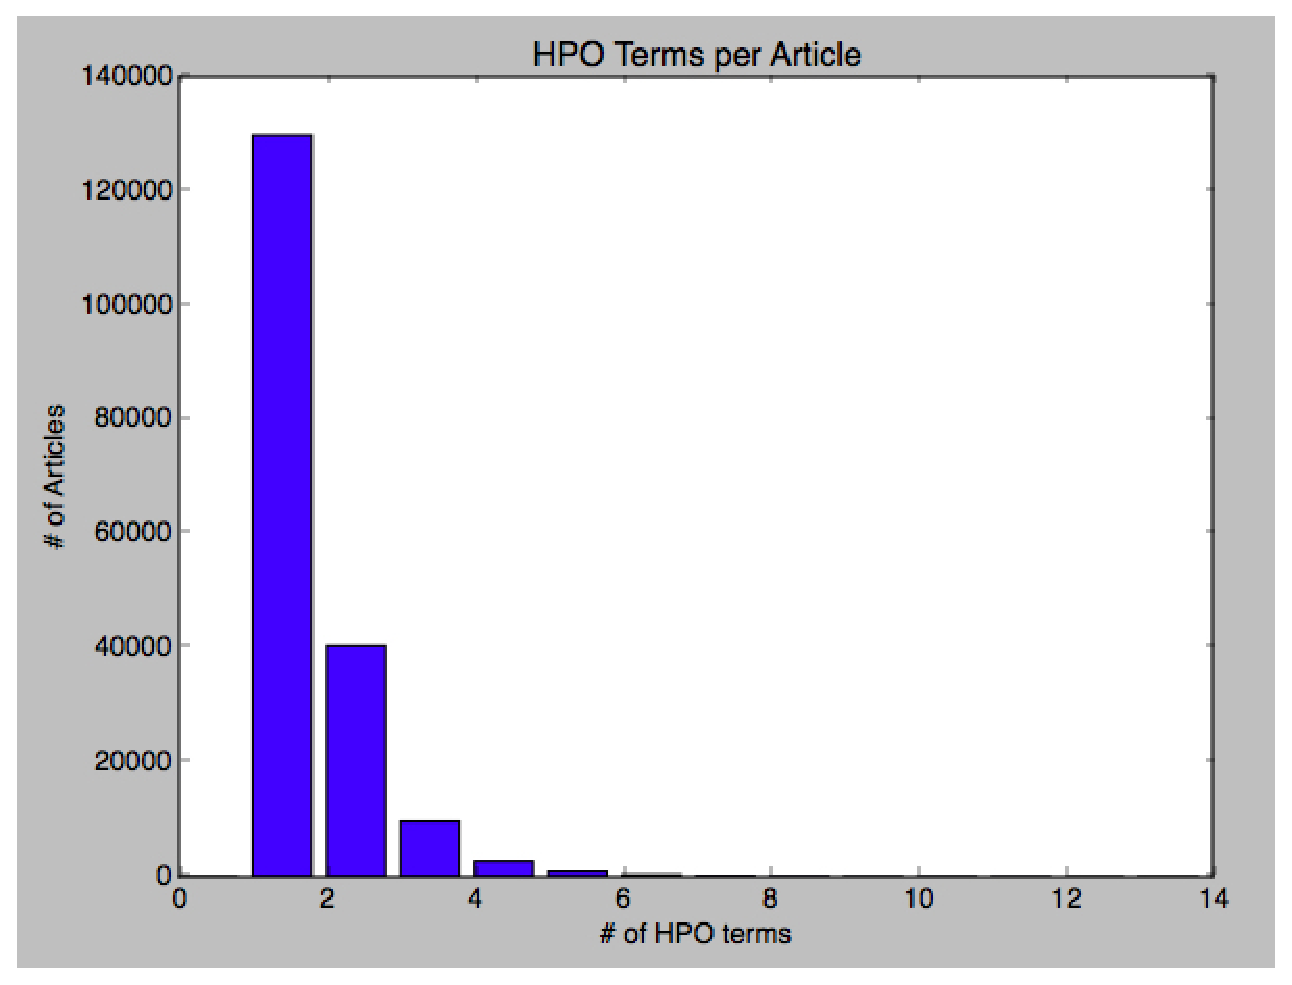
\includegraphics[width=8cm]{article-hpo}\\
 \small \textit{Fig 3.} This shows that most articles only have 1 HPO term tagged. 
\end{center}

\section{Logistic Regression}
My first attempt to tag articles with HPO terms was by using logistic regresison. I created a table of articles and HPO terms and did logistic regresison for an HPO term if it appeared in at least 100 articles. \\
\\
Logistic regression did not work to tag PubMed articles. It suffered from the fact that there were orders of magnitude more negative examples than positive examples. Even when I artificially balanced the number of positive and negative examples, it still did poorly. I also tried to increase the threshold––HPO terms would have to appear in 200, 500, 1,000 articles. The logistic regression weights essentially predicted only `negative' for an HPO term no matter what I did. 

\section{fastText}
Next, I tried fastText. fastText is a new algorithm from Facebook AI Research that performs text classification at levels comparable to neural networks without extremely long training times. A neural net could take hours or days to train, while fastText is done in a few minutes. fastText works by training a linear classifier on a `bag of words' and a `bag of n-grams' where n-grams are \textit{n} word long chunks that appear in the document. \\
\\
Again, I tresholded HPO terms so there was a large sample of documents labeled with a specific HPO term. I did a train-test split of 80\%-20\%. I only recently got fastText to work but I have some preliminary evaluations. 

\begin{center}
	\begin{tabular}{ | l | l | l | }
	\hline
	Threshold & Precision@1 & Recall@1 \\ \hline 
	100 & 35.54\% & 26.32 \% \\ \hline
	500 & 44.08\% & 34.51 \% \\ \hline 
	1,000 & 50.09\% & 39.81 \% \\ \hline
	5,000 & 48.50\% & 44.19 \% \\ \hline
	\end{tabular}
\end{center}

This is much better than logistic regression and believe fairly good for being `at 1' meaning we only consider the top HPO term returned by fastText. 
\subsection{Next steps for fastText}
I only recently got this up and running. There are several obvious next steps to improve my application of fastText. 
\begin{itemize}
\item Search the hyperparameter space
\item Do k-fold cross validation to estimate out of sample error 
\item Look at `precision at k' and `recall at k' for different \textit{k}
\end{itemize}

\section{Next steps}
If Andy and I decide that fastText is worth pursuing, I will do the next steps listed above for fastText. Another learning method to investigate is neural nets. This summer, I made some preliminary residual neural net structures. I can restart this and see how neural nets tackle this classification problem. \\ \\ 
After I determine the best possible classification method, I will apply my trained method to electronic medical records. I think that we should have the learning method portion of the project done by late May at the absolute latest, then testing on EMRs is a simple application. 


\bibliographystyle{ws-procs11x85}
\bibliography{ws-pro-sample}

\end{document}